% Plantoir house style: the finite-difference scaffold (the skill's section 10),
% a static example that needs nothing but LaTeX. Copy the tikzpicture into the
% FIRST table of the day that meets first or second differences, and change
% the numbers; later tables that day are plain. finite_differences.py beside
% this file writes the same picture for any table, if Python is available.
%
% This one is y = x^2 - 3 for x = -2 to 2. Every part that differs between
% the copies is written \qa{student}{answer}: the student copy works the first
% TWO first differences and the first second difference (so every value a
% worked line uses is already on the sheet), the rest are short blank rules
% that stop clear of the next column's arrows, and the answer key has every
% line. Compile with \def\showanswers{} in front (a "- Answers" wrapper) for
% the answer key. For a warmup that meets only first differences, keep the
% first column of arrows and drop the second, its heading included.
%
% Each arrow starts at the LOWER value and points UP to the one above it; its
% label is the whole subtraction, lower minus upper, negatives in brackets,
% lined up on the equals signs. Both columns of the table hold a negative
% value, so both are right-aligned with padding (anchor=east); a column with
% no negative value is centred (numc). Never on a quiz, test or practice test.
\documentclass[11pt]{article}
\usepackage[letterpaper, margin=0.75in, bottom=0.9in]{geometry}
\usepackage{lmodern}
\usepackage[T1]{fontenc}
\usepackage{amsmath}
\usepackage{tikz}
\setlength{\parindent}{0pt}

\newif\ifanswers
\ifdefined\showanswers \answerstrue \fi
\newcommand{\qa}[2]{\ifanswers #2\else #1\fi}

\begin{document}

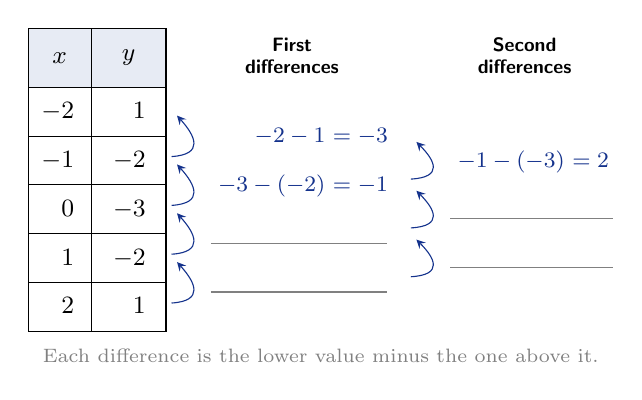
\begin{tikzpicture}[font=\small]
\definecolor{diffcol}{RGB}{20,50,140}
\definecolor{headfill}{RGB}{70,100,170}
\tikzset{num/.style={anchor=east, inner sep=0pt, text height=1.6ex, text depth=0.45ex},
  numc/.style={num, anchor=center},
  dif/.style={num, text=diffcol, font=\footnotesize},
  diffarrow/.style={diffcol, thin, -stealth}}
% The table of values: a shaded heading row, a full outer border, one ruled row for each x
\fill[headfill, fill opacity=0.13] (0,0) rectangle (1.75,-0.75);
\draw (0,0) rectangle (1.75,-3.850);
\draw (0.80,0) -- (0.80,-3.850);
\draw (0,-0.750) -- (1.75,-0.750);
\draw (0,-1.370) -- (1.75,-1.370);
\draw (0,-1.990) -- (1.75,-1.990);
\draw (0,-2.610) -- (1.75,-2.610);
\draw (0,-3.230) -- (1.75,-3.230);
\node at (0.400,-0.375) {$x$};
\node at (1.275,-0.375) {$y$};
% A column with any negative value is right-aligned with padding; one with none is centred
\node[num] at (0.59,-1.060) {$-2$};
\node[num] at (0.59,-1.680) {$-1$};
\node[num] at (0.59,-2.300) {$0$};
\node[num] at (0.59,-2.920) {$1$};
\node[num] at (0.59,-3.540) {$2$};
\node[num] at (1.50,-1.060) {$1$};
\node[num] at (1.50,-1.680) {$-2$};
\node[num] at (1.50,-2.300) {$-3$};
\node[num] at (1.50,-2.920) {$-2$};
\node[num] at (1.50,-3.540) {$1$};
% First differences: each arrow starts at the lower value and points up to the one above it;
% beside it, the subtraction: lower value minus the one above it
\node[font=\scriptsize\sffamily\bfseries, align=center, anchor=south] at (3.350,-0.700) {First\\differences};
\draw[diffarrow] (1.820,-1.630) .. controls (2.236,-1.604) and (2.124,-1.370) .. (1.890,-1.110);
\node[dif] at (3.780,-1.370) {$-2 - 1$}; \node[dif, anchor=west] at (3.780,-1.370) {${}= -3$};
\draw[diffarrow] (1.820,-2.250) .. controls (2.236,-2.224) and (2.124,-1.990) .. (1.890,-1.730);
\node[dif] at (3.780,-1.990) {$-3 - (-2)$}; \node[dif, anchor=west] at (3.780,-1.990) {${}= -1$};
\draw[diffarrow] (1.820,-2.870) .. controls (2.236,-2.844) and (2.124,-2.610) .. (1.890,-2.350);
\qa{\draw[gray] (2.320,-2.730) -- (4.560,-2.730);}{\node[dif] at (3.780,-2.610) {$-2 - (-3)$}; \node[dif, anchor=west] at (3.780,-2.610) {${}= 1$};}
\draw[diffarrow] (1.820,-3.490) .. controls (2.236,-3.464) and (2.124,-3.230) .. (1.890,-2.970);
\qa{\draw[gray] (2.320,-3.350) -- (4.560,-3.350);}{\node[dif] at (3.780,-3.230) {$1 - (-2)$}; \node[dif, anchor=west] at (3.780,-3.230) {${}= 3$};}
% Second differences: each arrow starts at the lower value and points up to the one above it;
% beside it, the subtraction: lower value minus the one above it
\node[font=\scriptsize\sffamily\bfseries, align=center, anchor=south] at (6.305,-0.700) {Second\\differences};
\draw[diffarrow] (4.860,-1.916) .. controls (5.276,-1.892) and (5.164,-1.680) .. (4.930,-1.444);
\node[dif] at (6.820,-1.680) {$-1 - (-3)$}; \node[dif, anchor=west] at (6.820,-1.680) {${}= 2$};
\draw[diffarrow] (4.860,-2.536) .. controls (5.276,-2.512) and (5.164,-2.300) .. (4.930,-2.064);
\qa{\draw[gray] (5.360,-2.420) -- (7.430,-2.420);}{\node[dif] at (6.820,-2.300) {$1 - (-1)$}; \node[dif, anchor=west] at (6.820,-2.300) {${}= 2$};}
\draw[diffarrow] (4.860,-3.156) .. controls (5.276,-3.132) and (5.164,-2.920) .. (4.930,-2.684);
\qa{\draw[gray] (5.360,-3.040) -- (7.430,-3.040);}{\node[dif] at (6.820,-2.920) {$3 - 1$}; \node[dif, anchor=west] at (6.820,-2.920) {${}= 2$};}
\node[font=\scriptsize, text=gray, anchor=north, text width=7.18cm, align=center] at (3.715,-3.950) {Each difference is the lower value minus the one above it.};
\end{tikzpicture}

\end{document}
